\documentclass{article}
% ready for submission
\usepackage[final]{neurips_2023}

% Language setting
% Replace `english' with e.g. `spanish' to change the document language
\usepackage[english]{babel}

% Set page size and margins
% Replace `letterpaper' with `a4paper' for UK/EU standard size
% \usepackage[letterpaper,top=2cm,bottom=2cm,left=3cm,right=3cm,marginparwidth=1.75cm]{geometry}

% Useful packages
\usepackage{amsmath}
\usepackage{graphicx}
\usepackage[colorlinks, linkcolor = black, citecolor=black]{hyperref}

\usepackage[utf8]{inputenc} % allow utf-8 input
\usepackage[T1]{fontenc}    % use 8-bit T1 fonts
%\usepackage{hyperref}       % hyperlinks
\usepackage{url}            % simple URL typesetting
\usepackage{booktabs}       % professional-quality tables
\usepackage{amsfonts}       % blackboard math symbols
\usepackage{nicefrac}       % compact symbols for 1/2, etc.
\usepackage{microtype}      % microtypography
\usepackage{xcolor}         % colors
\usepackage{hyperref}       % emails
\usepackage{marvosym}


\title{Binary Image Classification on Camera Trap Data for Detecting Sarcoptic Mange in Coyotes
}

\author{
  Moyinoluwa Famobiwo \\
  Department of Computing Science \\
  University of Alberta \\
  \href{mailto: famobiwo@ualberta.ca}{\texttt{famobiwo@ualberta.ca}} \\
  \And
  Steven Tang \\
  Department of Computing Science \\
  University of Alberta \\
  \href{mailto: stang5@ualberta.ca}{\texttt{stang5@ualberta.ca}} \\
  \AND 
  Tim Van Maren \\
  Department of Computing Science \\
  University of Alberta \\
  \href{mailto: vanmaren@ualberta.ca}{\texttt{vanmaren@ualberta.ca}} \\
  \And
  Akemi Izuko \\
  Department of Computing Science \\
  University of Alberta \\
  \href{mailto: izuko@ualberta.ca}{\texttt{izuko@ualberta.ca}} \\
  \AND
  Yongshan Yu \\
  Department of Computing Science \\
  University of Alberta \\
  \href{mailto: yongshan@ualberta.ca}{\texttt{yongshan@ualberta.ca}} \\
  \And 
  Sanad Masannat \\
  Department of Computing Science \\
  University of Alberta \\
  \href{mailto: sanad@ualberta.ca}{\texttt{sanad@ualberta.ca}} \\
}


\begin{document}
\maketitle


\begin{abstract}
  In recent decades, Convolutional Neural Networks (CNNs) have made remarkable progress in image processing domains, such as animal detection and skin disease classification. However, applying this technology to a novel domain involving both tasks presents new challenges that require exploration into Artificial Intelligence (AI) methods which can appropriately handle these constraints. This study explores the application of these technologies to a novel domain: detecting sarcoptic mange in coyotes using camera trap data. We conduct an extensive literature review, focusing on signs of animal skin diseases including mange, state-of-the-art neural network architectures, and advanced data pre-processing methods. We examine their strengths and weaknesses in addressing the unique challenges posed by this specific domain, providing insights into the difficulties of using camera trap images for wildlife skin disease detection and suggesting potential solutions to overcome these challenges. We propose a Residual Neural Network model and data pre-processing steps, which improve on the baseline expected cost provided by domain experts by 30\%, while also achieving a recall of 76\% on a locationally-disjoint test set. We further provide valuable insights and guidance regarding further application of ML in the domain of zoology and emphasize the importance of developing more robust models tailored to specific domains.
\end{abstract}


\section{Background}
Detecting sarcoptic mange in coyotes (Canis latrans) is a critical task for wildlife conservation and ecology. Sarcoptic mange, caused by the Sarcoptes scabei mite, is the predominant form of mange in coyotes. It leads to severe inflammation and symptoms such as fur loss, darkened skin, and self-inflicted wounds due to intense irritation [cite] and in worse cases, blindness, hypothermia and eventually death. As mange is highly contagious and often goes undetected until it is too late for recovery, it is essential to develop an efficient detection method to aid in timely intervention and treatment.
In response to the need for accurate sarcoptic mange detection in coyotes, we propose a binary image classification algorithm based on camera trap data to classify images into two categories: mange detected or mange not detected. Camera trapping, widely employed in wildlife observation and located in coyote habitats, captures consecutive images upon detecting motion, with approximately 30-second intervals between them. These camera traps provide valuable data for detecting mange in coyotes; however, the quality of the acquired data poses challenges to our research problem.
As shown in Figure 1, the trained neural network must detect mange in coyotes within challenging images, including situations where coyotes blend with their surroundings, images captured at night with poor illumination, blurry images due to motion, images with only a portion of the coyote visible, and images featuring multiple close-up coyotes. The limited amount of training data available for this task exacerbates these challenges. To address these issues, we explore various image processing techniques and approaches designed to improve the neural network's performance in detecting mange under a range of conditions.

\begin{figure}
\centering
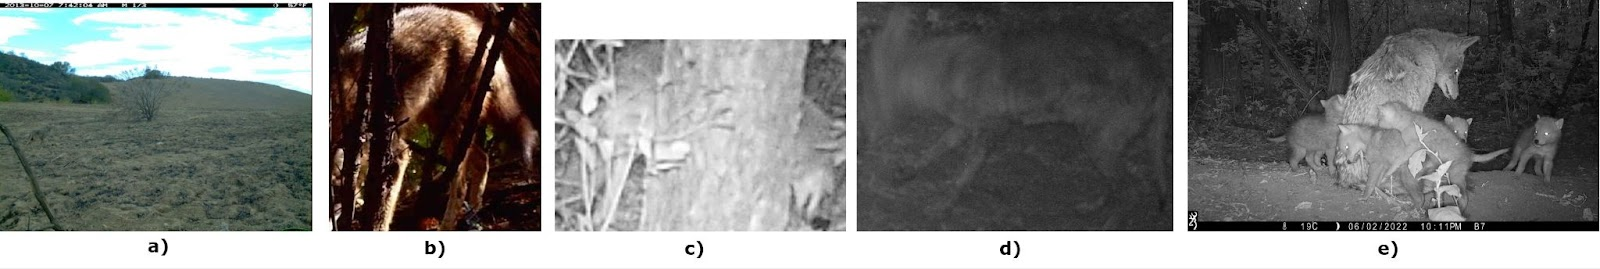
\includegraphics[width=1.0\textwidth]{fig1.jpeg}
\caption{\label{fig:fig1}Examples of challenging images from our datasets: a) The coyote blends with its surroundings. b) Image with only a portion of the coyote visible. c) Image captured at night with poor illumination. d) Image blurry due to coyote motion. e) Multiple close-up coyotes in one image.}
\end{figure}

By employing these techniques, we aim to develop an image classification algorithm capable of accurately detecting mange in coyotes. This will significantly improve the efficiency of mange detection, alleviate the workload of ecologists and wildlife conservationists, provide robust support for timely intervention and treatment of mange, and ultimately contribute to the health of coyote populations and the balance of ecosystems.

To showcase our research progress and findings, we have structured this report into several sections. We initiate with the task description in section 2 to establish the context of our study, followed by a literature review in section 3 that explores relevant works. Section 4 delves into our methodology, covering the various approaches and techniques we employed in pursuit of our objectives. Section 5 then outlines the metrics and evaluation methods used to assess our model's performance, providing a quantitative understanding of our results. Section 6 discusses our results in detail, addressing limitations and exploring potential avenues for future work. 

\section{Task Description}
Our task is to identify sarcoptic mange in coyotes from camera trap images by developing a binary classification algorithm. To illustrate the task more concretely, Figure 2 shows a simple example: given an input image of a coyote captured by a camera trap, our model makes a prediction and labels the image as either "mange detected" or "mange not detected" based on its previously learned knowledge. The output consists of a single class label, which corresponds to mange detected (1) or mange non detected (0).

\begin{figure}
\centering
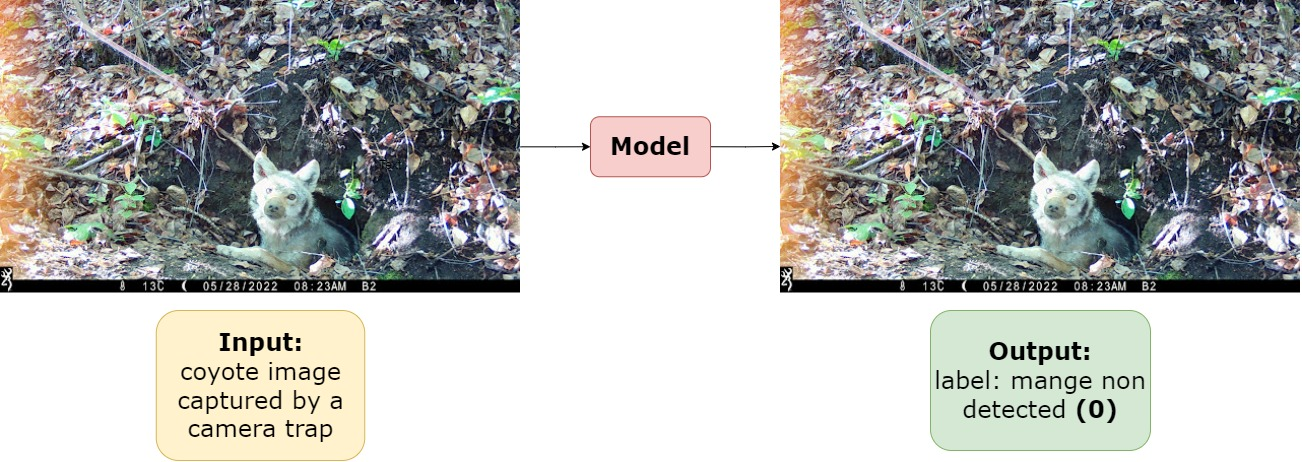
\includegraphics[width=1.0\textwidth]{fig2.jpeg}
\caption{\label{fig:fig2}A simple example of our task: the input is a coyote image captured by a camera trap, and the desired output is a single class label indicating mange detected (1) or mange not detected (0).}
\end{figure}

Our labeled dataset consists of approximately 15,000 images from camera traps in North America, specifically in Toronto, Chicago, and Edmonton. Around 2,000 (14\%) of these images are labeled as "mange detected." Human annotators determined the labels, which are provided in \verb|.csv| files alongside the images. The data set also includes timestamps and approximate locations for each image. To pre-process our data set, we employed techniques that may be beneficial for training, such as accurately cropping around coyotes using the MegaDetector and applying data augmentation to underrepresented categories to enhance the model's generalizability.

For training and evaluation of the models, we adopted a 5-fold cross-validation approach due to the relatively small size of our data set. This approach involves dividing the data set into five equal folds, which allows for more reliable performance estimates and facilitates the selection of the optimal model \cite{Berrar2019, Schaffer1993}. In each iteration of the validation process, four of the five folds are combined to form the training set, while the remaining fold serves as the validation set. This procedure is repeated five times, ensuring that each fold is used as a validation set exactly once, and the overall model performance is assessed by averaging the results from all five iterations.

To maintain the integrity of the validation process, we carefully ensured that the test and validation sets did not include images nearly identical to those in the training set. We achieved this by partitioning the set of images into subsets based on the camera used and the place of capture. All images within these subsets were then assigned to one of the training, validation, or testing sets. This separation ensures that our model is evaluated on its ability to generalize to unseen data based on the actual classification task of determining mange detected or mange not detected, rather than relying on memorizing the similar backgrounds present in images from the same location.

As a preliminary step to compare models, we evaluate precision and recall. However, our primary evaluation metric is the binary expected cost, as determined by our domain expert, which assesses the model's practical performance. We obtained the binary expected cost for each fold and then divided their sum by the number of folds to calculate the average binary expected cost for the model. The closer the value of the binary expected cost is to zero, the better the classification performance of the model.

\section{Methods}
In this section, we will discuss the approaches we took to address the challenges of detecting sarcoptic mange in coyotes, detailing the methods developed for each stage of our framework. Our method framework is divided into four main parts: data preprocessing, data augmentation, tabular features, and models.

\subsection{Data Pre-processing}
In our attempt to classify sarcoptic mange, we first needed to perform pre-processing on the data before employing any models. One of the critical challenges in detecting sarcoptic mange in coyotes using camera trap images is the presence of extraneous background information, which can potentially confuse the models and impact their performance. To address this issue, we decided to focus on cropping the images to emphasize the coyotes and minimize the influence of the background.

To achieve this, we used MegaDetector, an AI model specifically trained to detect objects including animals in camera trap images \cite{beery2019efficient, Fennell2022}. Developed by conservation biologists, MegaDetector streamlines the process of reviewing camera trap images by identifying objects of interest without classifying species. It helps to extract relevant information from the images, enabling researchers to focus on the images that matter.

Figure 3 provides a simple example of data preprocessing. In our study, MegaDetector was employed to identify the bounding box around the coyote in each image. After obtaining the bounding boxes, we cropped the images based on these boxes. This approach retained some background elements while emphasizing the coyote itself, allowing us to concentrate on the essential features for mange detection and minimize the impact of extraneous background information.

\begin{figure}
\centering
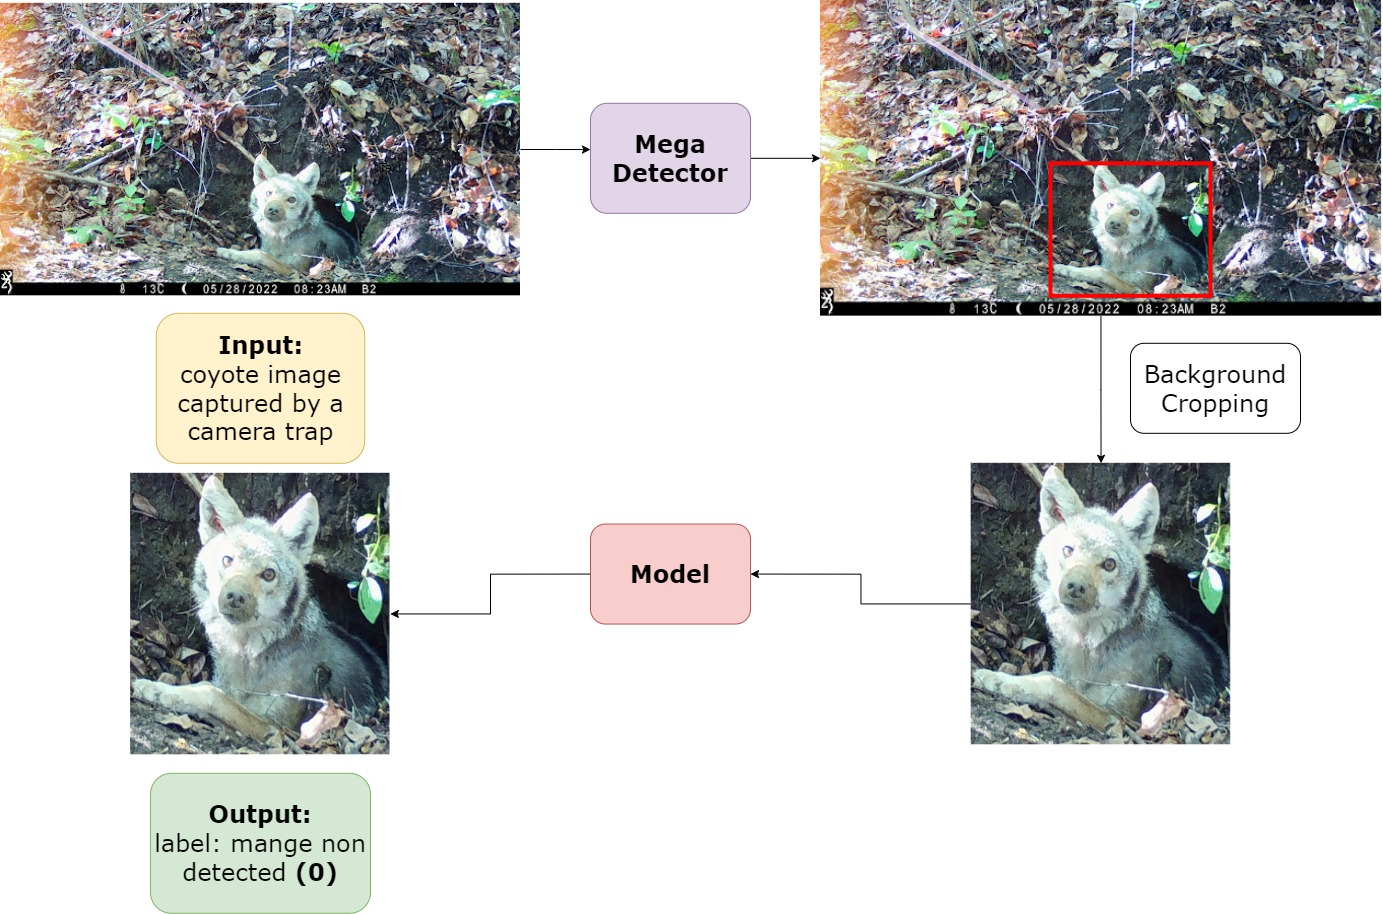
\includegraphics[width=1.0\textwidth]{fig3.jpeg}
\caption{\label{fig:fig3}An example of data preprocessing using MegaDetector. The original camera trap image of a coyote with extraneous background information (left) is processed by MegaDetector, which identifies the bounding box around the coyote in the image (indicated by the arrow). The cropped image based on the bounding box emphasizes the coyote and minimizes the influence of the background, allowing for better mange detection.}
\end{figure}

\subsubsection{MegaDetector}
Megadetector [cite] is an object detection model trained specifically on camera-trap images. It’s able to identify, label, and provide a bounding box for 3 categories: human, vehicle, and animal. An accurate bounding box reduces the noise in the image by quickly removing the majority of the image in most pictures. Before cropping our entire dataset, we used human labellers to evaluate how often the key features our domain experts said were important in identifying mange were contained in Megadetector’s bounding box. We found 82\% of bounding boxes for images with tails were able to capture over 50\% of the original tail within their bounds. However, when our model was trained using images cropped to Megadetector’s bounding box, the model consistently failed to attain the same recall scores, despite hyperparameter tuning on both models. See section 6 for a further discussion.
\subsection{Data Augmentation}
Data augmentation is a process in which we slightly modify the input images and then pass them into Neural Networks. This works because neural networks themselves are translationally invariant. Some common data augmentation methods include: Horizontal/Vertical Flip, Rotation of image, Gaussian Blurring, Random Cropping, Noise insertion and Colour jittering. Since the dataset we are working with is small, by using data augmentation, we can arbitrarily increase the size of our dataset for our neural network to train and test on. The expected result of this was improved accuracy. However, since different augmentations affect the data and accuracy differently, we needed to attempt multiple of the aforementioned augmentations and see which caused an increase in accuracy without causing the model to overfit. Thus, in our model, we used rotation, flipping and gaussian blurring.
\subsection{Data Programming}
While we were able to obtain 15,000 labeled images of labeled coyote images, we also found 40,000 unlabeled coyote camera trap images. Despite the prohibitive cost of labeling such massive amounts of images, the prospect of training on the vast quantities of unlabeled data was hard to give up. Unsupervised learning approaches can help here, specifically we considered data programming [cite]. This method uses a heuristic function developed from the process of labeling, as described by the domain experts, to “weakly” label the data. “Weak” labels are much noisier than their hand-labeled counterparts, though the sheer quantity of weak labels has been shown to help denoise the dataset as a whole.

Our domain experts [cite] provided the process they use for labeling coyotes for mange:
\begin{enumerate}
    \item If available, look at the thickness of the tail, one of the first signs of mange. The length to width ratio is very different between a healthy and furless tail.
    \item Look for bald patches of fur on the coyote’s back.
\end{enumerate}

However, the original paper only tests results on language models, a domain with significantly less noise than camera trap images. As such, our functions encoding the process described above were thrown off by the additional noise too much to be useful. For the first instance, our functions labeled almost all images as containing a mange-tail, due to picking up the twigs and branches in the background, instead of the tail. Further, when we labeled a random subset of our data, we found only 61\% of the images contained the coyote’s tail. For the second step, we attempted texture-based computer vision, though as found by other studies, most of our images had too low resolutions to accurately detect differences in fur texture[cite?]. In the end, the domain-knowledge encoding resulted in largely random labeling, so we were unable to use the unsupervised data.

\subsection{Vision Transformers}
Given the recent successes of the transformer model [cite] in the domain of language processing, computer vision research quickly adopted the architecture [cite some early paper].  Previous work using visual attention models showed promising results, particularly in classifying settings where the majority of the image is not relevant to the classification, such as housing numbers on streetview data [cite]. When applied to both the MegaDetector-cropped and uncropped camera trap images, we saw much higher recall rates with 49\% compared to the average 33\% on cropped images and 72\% compared to 50\% on uncropped images. Despite good performance on recall, the visual transformers had extremely high expected cost, often matching or even performing worse than the all-positive baseline. As our final evaluation metric is 5:1 expected cost, we chose to not pursue transformer methods any further.

\subsection{Models}

\section{Evaluation}
Our evaluation criteria consisted of expected cost, precision, recall and our chosen loss function was Weighted Binary Cross Entropy (WBCE). The formulas for precision and recall are the following:
\[Precision = \frac{TP}{TP+FP}\]
\[Recall = \frac{TP}{TP+FN}	    (1)\]     %Fix this     
Where TP indicates a True Positive, FP indicates a False Positive and FN indicates a false negative whose values we can get after performing our 5-fold cross validation and generating a confusion matrix. For our expected cost, we first assign false positives and false negatives a cost. False negatives are assigned a cost of 5 whereas false positives are assigned a cost of 1. Then we use the following formula: 
\[EC_5 = \frac{5FN + FP}{N}\]
and aim to minimize the output. The ideal expected cost here would be 0 but as we know that is unrealistic, our aim is to minimize this cost as much as we can. When our baseline model classifies all coyotes with no mange, we get an expected cost of 0.86. Within our tests, this was the highest we have gotten and our goal was to get a lower value.  The reason we assign the costs the way we have done is upon consultation with our domain expert, we learned that while a False Positive is not ideal and we should minimize it, a False Negative is even worse as we are letting an infected coyote roam free and infect others in the pack, thus leading to a higher cost in the future. We were also informed that the ideal ratio of false positives to false negatives was a 1:5 ratio. Using that, we decided to use the aforementioned expected cost formula.

For our loss function, we decided to use weighted binary cross entropy. WBCE is a loss metric in which a parameter alpha is placed on  regular Binary Cross Entropy loss in which said parameter will penalize false positives or negatives more depending on the value of the parameter. In our case, we want to penalize false negatives more so we set the alpha value to a value lower than 1. There were a few reasons as to why we chose to use WBCE. The first reason is that in our tests against other weight loss functions, it proved to be the best out of all the other metrics. The second major reason is that the idea of weighted BCE matched the aforementioned goal of attaining a 1:5 ratio of False Positives and Negatives in which we are penalized more for false negatives. Below is the formula for weighted binary cross entropy loss:
\[
-\frac{1}{M}\sum_{m-1}^{M}\alpha \cdot y \cdot \log(y(\hat{z}))-(1-y)\cdot\log(y(\hat{z})) 
\]
in which $\log(y(\hat{z}))$ is the output of the model, $\alpha$ is the weight parameter and the training weight.


\section{Results}

\section{Discussion}

\subsection{Conclusion}

\subsection{Future Research}
Given the comparative scarcity of labeled data and the difficulty associated with unsupervised learning in such a noisy setting, we suggest further research consider co-learning and other semi-supervised learning methods to take advantage of this readily available data.

\section{Acknowledgements}
We would like to thank our domain experts Sage Raymond, Tiziana [surname], Maureen [surname] and Mason [surname], who provided us with their own invaluable data and experience to guide us along this journey. We’re also grateful to the University of Alberta Autonomous Robotic Vehicle Project club for allowing us to use their server for all our model training and storage.
\clearpage
\bibliographystyle{unsrt}
\bibliography{reference}

\end{document}
